%    Copyright 2023 Bastien Veuthey, HES-SO//Bachelor
%
% Licensed under the Apache License, Version 2.0 (the "License");
% you may not use this file except in compliance with the License.
% You may obtain a copy of the License at
%
% http://www.apache.org/licenses/LICENSE-2.0
%
% Unless required by applicable law or agreed to in writing, software
% distributed under the License is distributed on an "AS IS" BASIS,
% WITHOUT WARRANTIES OR CONDITIONS OF ANY KIND, either express or implied.
% See the License for the specific language governing permissions and
% limitations under the License.

% =============================================================================
% | HES-SO//Master - Thesis project report template                           |
% |                                                                           |
% | Originally based on the EPFL and Marc Demierre template, with many        |
% | adjustements                                                              |
% | Source : https://github.com/bastienvty/hesso-template-latex               |
% =============================================================================

% Document settings
\documentclass[a4paper,11pt,fleqn]{book}
%\documentclass[a4paper,11pt,fleqn,openany]{book} % To begin directly the chapter's page
\usepackage[utf8]{inputenc}
\usepackage[T1]{fontenc}
\usepackage[french,english]{babel}

% -----------------------------------------------------------------------------
% Preamble
% -----------------------------------------------------------------------------
% =============================================================================
% | Thesis metadata                                                           |
% =============================================================================

% Thesis info
\newcommand{\ThesisTitle}{[ThesisTitle]}
\newcommand{\ThesisSubject}{[ThesisSubject]}
\newcommand{\Orientation}{Computer Science}
\newcommand{\Keywords}{keyword1, keyword2, keyword3}
\newcommand{\Keywordsfr}{motclé1, motclé2, motclé3}

% Author
\newcommand{\AuthorFirstName}{[FirstName]}
\newcommand{\AuthorLastName}{[LastName]}
\newcommand{\AuthorEmail}{[user@domain.com]}
\newcommand{\Author}{\AuthorFirstName\ \AuthorLastName}

% Advisor
\newcommand{\AdvisorFirstName}{[FirstName]}
\newcommand{\AdvisorLastName}{[LastName]}
\newcommand{\AdvisorSchool}{[School]}
\newcommand{\AdvisorResearchUnit}{[ResearchUnit]}
\newcommand{\Advisor}{\AdvisorFirstName\ \AdvisorLastName}

% Main expert
\newcommand{\ExpertFirstName}{[FirstName]}
\newcommand{\ExpertLastName}{[LastName]}
\newcommand{\Expert}{\ExpertFirstName\ \ExpertLastName}
\newcommand{\ExpertLab}{[Lab/Company]}

% Dean
\newcommand{\Dean}{Prof. X}

% Place (for date and place)
\newcommand{\Date}{\today}
\newcommand{\Place}{Fribourg}         % your project data
% ==================
% Template settings
% ==================

% General tools
% -------------
\usepackage{etoolbox}
\usepackage{algorithm}
\usepackage{algpseudocode}

% Page style
% ----------
\usepackage[margin=3cm, left=3.5cm, right=3.5cm, twoside=true]{geometry}
\usepackage{fancyhdr}
\setlength{\headheight}{14pt}
\renewcommand{\sectionmark}[1]{\markright{\thesection\ #1}}
\pagestyle{fancy}

% Standard pages (inside chapters)
\fancyhf{}
\renewcommand{\headrulewidth}{0.4pt}
\renewcommand{\footrulewidth}{0pt}
\fancyhead[OR]{\bfseries \nouppercase{\rightmark}}
\fancyhead[EL]{\bfseries \nouppercase{\leftmark}}
\fancyfoot[EL,OR]{\thepage}

% First page of chapters
\fancypagestyle{plain}{
	\fancyhf{}
	\renewcommand{\headrulewidth}{0pt}
	\renewcommand{\footrulewidth}{0pt}
	\fancyfoot[EL,OR]{\thepage}
}

% Imports for external PDFs
\fancypagestyle{addpagenumbersforpdfimports}{
	\fancyhead{}
	\renewcommand{\headrulewidth}{0pt}
	\fancyfoot{}
	\fancyfoot[RO,LE]{\thepage}
}

% Use empty style for page when clearing double pages
\def\cleartoodd{%
	\clearpage%
	\ifodd\value{page}\else\mbox{}\thispagestyle{empty}\newpage\fi%
}

\def\clearchap{%
	\ifodd\value{page}\else\mbox{}\thispagestyle{empty}\fi%
}

% \cleardoublepage replaced by \cleartoodd
\let\origdoublepage\cleardoublepage
\renewcommand{\cleardoublepage}{%
	\cleartoodd%
}

% Fonts
% -----

% Helvetica (Arial used in the MSE Word template)
\usepackage{helvet}

% Math
% ----
\usepackage{amsmath}  % better math

% Floats and figures
% ------------------
\usepackage{float}
\usepackage{newfloat}          % floats
\usepackage[twoside]{caption}  % captions
\usepackage{subcaption}        % subcaptions
\usepackage[section]{placeins} % allows to put float barriers

% Float captions in italics, with label in margin
\DeclareCaptionLabelFormat{title}{#1 #2}
\DeclareCaptionLabelFormat{hangout}{\llap{#1 #2\hspace{5mm}}}
\captionsetup{
	format=hang,
	%labelformat=hangout,
	singlelinecheck=true,
	font={it}
}

% Caption with source for figure
% TODO: improve this to use square brackets like the normal "caption"
\newcommand*{\captionsource}[3]{%
	\caption[{#1}]{%
		#2%
		
		\scriptsize{\textbf{Source:} #3}%
	}%
}

% Tables
% ------
\usepackage{booktabs} % much better tables
\usepackage{multirow} % allows to fuse rows
\usepackage{array}    % manipulate array
\usepackage{tabularx} % better tables
\usepackage{makecell} % multilined columns

% Define new tabularx column types:
%  - R: streteched right aligned
%  - C: stretched centered
%  - N: left aligned, specified space
\newcolumntype{R}[1]{>{\raggedleft\arraybackslash}p{#1}}%
\newcolumntype{C}[1]{>{\centering\arraybackslash}p{#1}}%
\newcolumntype{L}[1]{>{\raggedright\arraybackslash}p{#1}}%

% Set row height multiplicator to provide more breathing space
\renewcommand{\arraystretch}{1.3} 
%\renewcommand\theadalign{bc}
%\renewcommand\theadfont{\bfseries}
%\renewcommand\theadgape{\Gape[4pt]}
%\renewcommand\cellgape{\Gape[4pt]}

% Bibliography
% -------------------

% Use biber, with numeric style and no sorting (citation order)
\usepackage[
backend=biber,
style=numeric,
sorting=none,
bibencoding=auto
]{biblatex}
\addbibresource{structure/3-tail/bibliography.bib}


% Tables of contents, figures, tables and listings
% ------------------------------------------------
\usepackage{tocloft}
\usepackage{enumerate}
\newlistof{listing}{lol}{List of Listings}
\setcounter{tocdepth}{1} % Depth to 'section'
\setlength{\cftfigindent}{0pt}  % remove indentation from figures in lof
\setlength{\cftfignumwidth}{1cm}
\setlength{\cfttabindent}{0pt}  % remove indentation from tables in lot
\setlength{\cfttabnumwidth}{1cm}
\setlength{\cftlistingindent}{0pt}
\setlength{\cftlistingnumwidth}{1cm}

% Mini tables of contents
% -----------------------
\usepackage{minitoc}

% no "Contents" title
\mtcsettitle{minitoc}{Contents} 

% Layout
\setlength{\mtcindent}{-0.5em}
\mtcsetoffset{minitoc}{-1em}

% Spacing above and below table
\mtcsetfeature{minitoc}{before}{\vspace{0.5cm}}
\mtcsetfeature{minitoc}{after}{\vspace{-0.25cm}}
\renewcommand{\mtifont}{\sffamily\bfseries\large}

% Colors & graphics
% -----------------
\usepackage[table, svgnames, dvipsnames]{xcolor}      % colors
\usepackage[pdftex]{graphicx}   % graphics importing
\graphicspath{{structure/figures/}}
\definecolor{gray80}{gray}{0.80}


% Code and syntax highlighting
% ----------------------------
\usepackage[newfloat]{minted}   % code highlighting

% Typography
% ----------
\usepackage{csquotes}                    % paragraph indentation and spacing
\usepackage[defaultlines=3,all]{nowidow} % avoid widows and orphans
\usepackage{microtype}                   % typographic improvements
\usepackage{parskip}                     % No indent and auto-space between paragraphs
\usepackage[super]{nth}

\usepackage{paralist}
\usepackage{enumitem}
\setlist{after=\vspace{\baselineskip}}

% Section and chapters headings
% -----------------------------
\usepackage[explicit]{titlesec} % titles formatting
%\usepackage{titletoc} % titles formatting in ToC etc
%\usepackage{sectsty}  % sectioning commands

% -- Chapters --
% Remove "Chapter N" and use a sans-serif font

% Set layout lengths
\setlength{\headheight}{8mm}
\setlength{\footskip}{1.5cm}
\addtolength{\textheight}{-.5cm}

\titlespacing{\chapter}{-5mm}{-10mm}{3mm}
\titlespacing{\section}{-5mm}{3mm}{2mm}
\titlespacing{\subsection}{-5mm}{2mm}{2mm}
\titlespacing{\subsubsection}{-5mm}{2mm}{0mm}


%\titleformat{\chapter}[block]
%{\Huge}
%{\thechapter\hspace{12pt}\textcolor{gray80}{|}\hspace{12pt}}
%{0pt}
%{\Huge\bfseries}

\titleformat{\chapter}{\Huge\bfseries}{\llap{\thechapter\hspace{12pt}\textcolor{gray80}{|}}}{0mm}{%
	\hfill\begin{minipage}[t]{\dimexpr\textwidth}\raggedright#1\end{minipage}%
}
\titleformat{\section}{\Large\bfseries}{\llap{\thesection}}{0mm}{%
	\hfill\begin{minipage}[t]{\dimexpr\textwidth}\raggedright#1\end{minipage}%
}
\titleformat{\subsection}{\large \bfseries}{\llap{\thesubsection}}{0mm}{%
	\hfill\begin{minipage}[t]{\dimexpr\textwidth}\raggedright#1\end{minipage}%
}
\titleformat{\subsubsection}{\bfseries}{\llap{\thesubsubsection}}{0mm}{%
	\hfill\begin{minipage}[t]{\dimexpr\textwidth}\raggedright#1\end{minipage}%
}

% Misc
% ------
\usepackage{lipsum}    % filler text
\usepackage{blindtext} % random text
\usepackage{lscape}    % easy landscape pages
\usepackage{pdflscape} % landscape pages for PDFs

% Allow email typesetting
\newcommand{\email}[1]{%
	\href{mailto:#1}{\textit{#1}}%
}

% TODO NOTES
% -----------
\usepackage{todonotes}

% References
% -----------
\usepackage{url}
%\usepackage{varioref}

% pdf metadata
\usepackage[
	pdfauthor={\Author},
	pdftitle={\ThesisTitle},
	pdfsubject={\ThesisSubject},
	pdfkeywords={\Keywords}
	pdfduplex=DuplexFlipLongEdge]{hyperref}
	
%\usepackage{cleveref}
		
% Hyperlinks
\hypersetup{
	colorlinks=true,
	linkcolor=black,
	citecolor=black,
	filecolor=black,
	urlcolor=black,
}
\providecommand*{\listingautorefname}{Listing}

% Chapters on same page
\usepackage{etoolbox}
\makeatletter
\patchcmd{\chapter}{\if@openright\cleardoublepage\else\clearpage\fi}{}{}{}
\makeatother

% Glossary
% --------
\usepackage[toc,section=chapter]{glossaries}
% Terms
% -----
% format:  \newglossaryentry{<label>}{<settings>}
% example: \newglossaryentry{computer}
%{
%	name=computer,
%	description={is a programmable machine that receives input,
%		stores and manipulates data, and provides
%		output in a useful format}
%}
\newglossaryentry{nosql}
{
	name=NoSQL,
	description={Database not using the relational model and the \acrshort{sql} language}
}

% Acronyms
% --------
% format:  \newacronym{<label>}{<abbrv>}{<full>}
% example: \newacronym{lvm}{LVM}{Logical Volume Manager}
% plural:  \newacronym[longplural={Frames per Second}]{fpsLabel}{FPS}{Frame per Second}

\newacronym{api}{API}{Application Programming Interface}

\newacronym{cep}{CEP}{Complex Event Processing}
\newacronym{ci}{CI}{Continuous Integration}
\newacronym{cqrs}{CQRS}{Command Query Responsibility Segregation}
\newacronym{crud}{CRUD}{Create-Read-Update-Delete}

\newacronym{dag}{DAG}{Directed Acyclic Graph}
\newacronym{dsl}{DSL}{Domain Specific Language}

\newacronym{eca}{ECA}{Event Condition Action}
\newacronym{elk}{ELK}{Elasticseach Logstash and Kibana}
\newacronym{efk}{EFK}{Elasticseach Fluentd and Kibana}
\newacronym{epa}{EPA}{Event Processing Agent}
\newacronym{epn}{EPN}{Event Processing Network}

\newacronym{gelf}{GELF}{Graylog Extended Log Format}
\newacronym{ge}{GE}{Generic Enabler}

\newacronym{ide}{IDE}{Integrated Development Environment}
\newacronym{iot}{IoT}{Internet of Things}

\newacronym{jar}{JAR}{Java ARchive}
\newacronym{jmx}{JMX}{Java Management Extensions}
\newacronym{json}{JSON}{JavaScript Object Notation}
\newacronym{jvm}{JVM}{Java Virtual Machine}

\newacronym{poc}{PoC}{Proof of Concept}

\newacronym{rest}{REST}{Representational state transfer}
\newacronym{rest_markup}{reST}{reStructuredText}
\newacronym{rpc}{RPC}{Remote Procedure Call}

\newacronym{sql}{SQL}{Structured  Query Language}

\newacronym{uuid}{UUID}{Universally Unique Identifier}
\newacronym{uri}{URI}{Universal Resource Identifier}

\makeglossaries

    % template settings
% ===========================================
% = Codestyles for minted syntax highlighting
% ===========================================

% How to configure a language with minted:
% Language
%\newminted{language}{frame=single, framesep=6pt, breaklines=true, fontsize=\scriptsize, escapeinside=||}
%\newmintedfile{language}{frame=single, framesep=6pt, breaklines=true, fontsize=\scriptsize}
%\usemintedstyle[language]{pastie} % optional (ref: https://www.overleaf.com/learn/latex/Code_Highlighting_with_minted#Reference_guide)

% How to use (replace 'java' with language name):
% - code blocks:
%     \begin{javacode}
%     CODE
%     \end{javacode}
% - files:
%     full: \javafile{PATH}
%     extract: \javafile[startline=x, endline=y]{PATH}

% Java
\newminted{java}{frame=single, framesep=6pt, breaklines=true, fontsize=\scriptsize}
\newmintedfile{java}{frame=single, framesep=6pt, breaklines=true, fontsize=\scriptsize}
%TC:group javacode 0 0

% C
\newminted{c}{frame=single, framesep=6pt, breaklines=true, fontsize=\scriptsize}
\newmintedfile{c}{frame=single, framesep=6pt, breaklines=true, fontsize=\scriptsize}
%TC:group ccode 0 0

% CPP
\newminted{cpp}{frame=single, framesep=6pt, breaklines=true, fontsize=\scriptsize}
\newmintedfile{cpp}{frame=single, framesep=6pt, breaklines=true, fontsize=\scriptsize}
%TC:group cppcode 0 0

% Scala
\newminted{scala}{frame=single, framesep=6pt, breaklines=true, fontsize=\scriptsize}
\newmintedfile{scala}{frame=single, framesep=6pt, breaklines=true, fontsize=\scriptsize}
%TC:group scalacode 0 0

% Clojure
\newminted{clojure}{frame=single, framesep=6pt, breaklines=true, fontsize=\scriptsize}
\newmintedfile{clojure}{frame=single, framesep=6pt, breaklines=true, fontsize=\scriptsize}
%TC:group clojurecode 0 0

% Python
\newminted{python}{frame=single, framesep=6pt, breaklines=true, fontsize=\scriptsize}
\newmintedfile{python}{frame=single, framesep=6pt, breaklines=true, fontsize=\scriptsize}
%TC:group pythoncode 0 0

% Sql
\newminted{sql}{frame=single, framesep=6pt, breaklines=true, fontsize=\scriptsize}
\newmintedfile{sql}{frame=single, framesep=6pt, breaklines=true, fontsize=\scriptsize}
%TC:group sqlcode 0 0

% Json
\newminted{json}{frame=single, framesep=6pt, breaklines=true, fontsize=\scriptsize}
\newmintedfile{json}{frame=single, framesep=6pt, breaklines=true, fontsize=\scriptsize}
%TC:group jsoncode 0 0

% Yaml
\newminted{yaml}{frame=single, framesep=6pt, breaklines=true, fontsize=\scriptsize}
\newmintedfile{yaml}{frame=single, framesep=6pt, breaklines=true, fontsize=\scriptsize}
\usemintedstyle[yaml]{pastie}
%TC:group yamlcode 0 0

% Rust
\newminted{rust}{frame=single, framesep=6pt, breaklines=true, fontsize=\scriptsize}
\newmintedfile{rust}{frame=single, framesep=6pt, breaklines=true, fontsize=\scriptsize}
\usemintedstyle[rust]{trac}
%TC:group rustcode 0 0

% Go
\newminted{go}{frame=single, framesep=6pt, breaklines=true, fontsize=\scriptsize}
\newmintedfile{go}{frame=single, framesep=6pt, breaklines=true, fontsize=\scriptsize}
\usemintedstyle[go]{manni}
%TC:group gocode 0 0

% Plain text
\newminted{text}{frame=single, framesep=6pt, breaklines=true, breakanywhere, fontsize=\scriptsize, escapeinside=||} % example: |\colorbox{green}{highlight code}|
\newmintedfile{text}{frame=single, framesep=6pt, breaklines=true, breakanywhere, fontsize=\scriptsize}
%TC:group textcode 0 0

% Shell
\newminted{shell}{frame=single, framesep=6pt, breaklines=true, breakanywhere, fontsize=\scriptsize}
\newmintedfile{shell}{frame=single, framesep=6pt, breaklines=true, breakanywhere, fontsize=\scriptsize}
%TC:group shellcode 0 0

% Console
\newminted{console}{frame=single, framesep=6pt, breaklines=true, breakanywhere, fontsize=\scriptsize}
\newmintedfile{console}{frame=single, framesep=6pt, breaklines=true, breakanywhere, fontsize=\scriptsize}
%TC:group consolecode 0 0

% Base Make
\newminted{basemake}{frame=single, framesep=6pt, breaklines=true, fontsize=\scriptsize}
\newmintedfile{basemake}{frame=single, framesep=6pt, breaklines=true, fontsize=\scriptsize}
%TC:group basemakecode 0 0

% Assembly
\newminted{gas}{frame=single, framesep=6pt, breaklines=true, fontsize=\scriptsize}
\newmintedfile{gas}{frame=single, framesep=6pt, breaklines=true, fontsize=\scriptsize}
%TC:group gascode 0 0       % code styles for minted
% ========================
% = TODO: Document
% ========================

% Marc's font stack
\usepackage{cmbright}       % Sans serif
\usepackage{sourcecodepro}  % Monospace
\usepackage{lmodern}
\renewcommand{\familydefault}{\sfdefault}  % your custom packages etc

\begin{document}
% -----------------------------------------------------------------------------
% Front matter
% -----------------------------------------------------------------------------
\frontmatter

\dominitoc

% ==========================================================================
% = HES-SO Master thesis title page (modeled after Word template, 2016-2017)
% ==========================================================================

\begin{titlepage}
\newgeometry{margin=2.5cm}
{\fontfamily{phv}\fontseries{mc}\selectfont
	\begin{flushright}
		\begin{minipage}{0.5\textwidth}
			\begin{flushleft}
				
\includegraphics[width=0.9\textwidth]{img/mse_logo}
			\end{flushleft}
		\end{minipage}%
		\begin{minipage}{0.5\textwidth}
			\begin{flushright}
				
\includegraphics[width=0.6\textwidth]{img/hesso_logo}
			\end{flushright}
		\end{minipage}
		\begin{flushleft}
			\footnotesize
			Master of Science HES-SO in Engineering \\
			Av. de Provence 6 \\
			CH-1007 Lausanne
		\end{flushleft}
		~\\[0.5cm]
		
		{
		\Huge Master of Science HES-SO in Engineering\\[0.5cm]
		}
		
		{
		\LARGE Orientation: \Orientation\\[0.5cm]
		~\\[1cm]
		}
		% Title
		{
			\Huge
			\ThesisTitle \\[1.5cm]
		}
		{
			\large
			Author:\\[-0.3cm]
			\Huge \Author \\[0.8cm]
		}
		{
			\large
			Under the supervision of: \\
			\Advisor \\
			\AdvisorResearchUnit \\[0.5cm]
		}
		{
			\large
			External expert: \\
			\Expert
		}
		\vfill
		
		% Bottom of the page
		{\large \Place, HES-SO//Master, \Date}
		
	\end{flushright}
}
\restoregeometry
\end{titlepage}





% Page for student info and signatures
\cleardoublepage
\chapter*{Information about this report}

\vspace{\fill}

\textbf{Contact information}

\begin{tabularx}{\textwidth}{L{2.5cm}X}
	Author:	 & \AuthorFirstName \AuthorLastName \\
	& Bachelor Student \\
	& HES-SO//Bachelor \\
	& Switzerland \\
	Email: & \email{\AuthorEmail}
\end{tabularx}

\vspace{\fill}

\textbf{Declaration of honor}

{\renewcommand{\arraystretch}{2}
\begin{tabularx}{\textwidth}{L{2.5cm}X}
	& I, undersigned, \Author, hereby declare that the work submitted is 
	the result of a personal work. I certify that I have not resorted to 
	plagiarism or other forms of fraud. All sources of information used and the 
	author quotes were clearly mentioned. \\
	Place, date: & \underline{\hspace{7cm}} \\ 
	Signature: & \underline{\hspace{7cm}}
\end{tabularx}
}

\vspace{\fill}

\textbf{Validation}

Accepted by the HES-SO//Bachelor (Switzerland, Fribourg) on a proposal from:

\vspace{0.5cm}

\Advisor, Thesis project advisor

\Expert, \ExpertLab, Main expert

\vspace{1cm}

Place, date: \underline{\hspace{8cm}}

\vspace{3cm}

{ \renewcommand{\arraystretch}{1.5}
\begin{tabularx}{\textwidth}{X X}
	\Advisor  & \Dean\\ 
	Advisor   & Dean, HES-SO//Master\\
\end{tabularx}
}

% French + English abstracts
\clearpage
% English abstract
\chapter*{Abstract}
%\markboth{Abstract}{Abstract}
\addcontentsline{toc}{chapter}{Abstract (English/Français)} % adds an entry to the table of contents

\lipsum[1-2]

\vskip0.5cm
\textbf{Key words:} 
\Keywords


% French abstract
\clearpage
\begin{otherlanguage}{french}
\chapter*{Résumé}
%\markboth{Résumé}{Résumé}

\lipsum[1-2]

\vskip0.5cm
\textbf{Mots clés:} 
\Keywordsfr
\end{otherlanguage}



% Dedication (maybe for another time...)
\clearpage
\thispagestyle{empty}


\vspace*{3cm}

\begin{raggedleft}
    	Sometimes a scream is better than a thesis.\\
     --- Manfred Eigen\\
\end{raggedleft}

\vspace{4cm}

\begin{center}
    To my parents\dots
\end{center}




% Acknowledgments (your dedication etc)
\clearpage
\chapter*{Acknowledgments}
\markboth{Acknowledgements}{Acknowledgements}
\addcontentsline{toc}{chapter}{Acknowledgements}

% -- Your text goes here --
\lipsum[1-2]


% Preface (to be written by someone else)
\clearpage
\chapter*{Preface}
\markboth{Preface}{Preface}
\addcontentsline{toc}{chapter}{Preface}
% put your text here
A preface is not mandatory. It would typically be written by some other person (eg your thesis director).

\lipsum[1-2]

\bigskip
 
\noindent\textit{Fribourg, 21 March 2022}
\hfill T.~D.


% Table of contents
\clearpage
\phantomsection
\addcontentsline{toc}{chapter}{Contents}
\tableofcontents

% List of figures
\clearpage
\phantomsection
\addcontentsline{toc}{chapter}{List of Figures}
\listoffigures

% List of tables
\phantomsection
\addcontentsline{toc}{chapter}{List of Tables}
\listoftables

% List of listings
\phantomsection
\addcontentsline{toc}{chapter}{List of Listings}
\listoflistings

% Restore paragraphs
\setlength{\parskip}{1em}

% Bold fonts for sections in minitoc
\renewcommand{\cftsecfont}{\sffamily\bfseries}
\renewcommand{\cftsecleader}{\sffamily\bfseries\cftdotfill{\cftdotsep}}
\renewcommand{\cftsecpagefont}{\sffamily\bfseries}


% -----------------------------------------------------------------------------
% Main matter
% -----------------------------------------------------------------------------
\mainmatter

% Chapters
\setcounter{mtc}{7} % Help minitoc skip the front matter chapters
\chapter{Introduction}
\label{chap:introduction}

% -----------------------------------------------------------------------------
\section{Context}

\lipsum[1]

% -----------------------------------------------------------------------------
\section{Objectives}

\lipsum[1]

% -----------------------------------------------------------------------------
\section{Structure of this report}

\lipsum[1]


\chapter{Analysis}
\label{chap:analysis}

\lipsum[1]

\minitoc

\newpage

% -----------------------------------------------------------------------------
This chapter shows example of picture and also serves to populate the different lists: list of figures, list of tables, bibliography, and glossary.

\section{Tables}

This section contains an examples of table: \autoref{tab:esempio} and 

\begin{table}[H]
	\centering
	\begin{tabular}{ccc}
		\toprule
		name & weight & food \\ 
		\midrule
		mouse	& 10 g	& cheese \\
		cat	& 1 kg	& mice \\
		dog	& 10 kg	& cats \\
		\bottomrule 
	\end{tabular}
	\caption[A floating table]{A floating table.}
	\label{tab:esempio}
\end{table}

\chapter{Milestones}
\label{chap:milestones}

The project consists of several milestones along the way to lay the foundation for its progress.

\begin{table}[H]
    \centering
    \rowcolors{1}{Lavender!80!gray}{white}
	\begin{tabular}{|L{2.5cm}|L{2.5cm}|C{3cm}|}
		\hline
		\rowcolor{lightgray} \textbf{\large{Name}} & \textbf{\large{Weight}} & \textbf{\large{Food}} \\
		\hline
		mouse & 10g & cheese \\
		\hline
            cat & 1kg & mice \\
		\hline
            dog & 10kg & cats \\
		\hline
	\end{tabular}
	\caption{A pretty table}
\end{table}

\section{Figures}

This section contains examples of figures: \autoref{fig:galleria}, \autoref{fig:lorem}, \autoref{fig:ipsum}, \autoref{fig:dolor}, \autoref{fig:sit}

\begin{figure}[H] 
	\centering 
	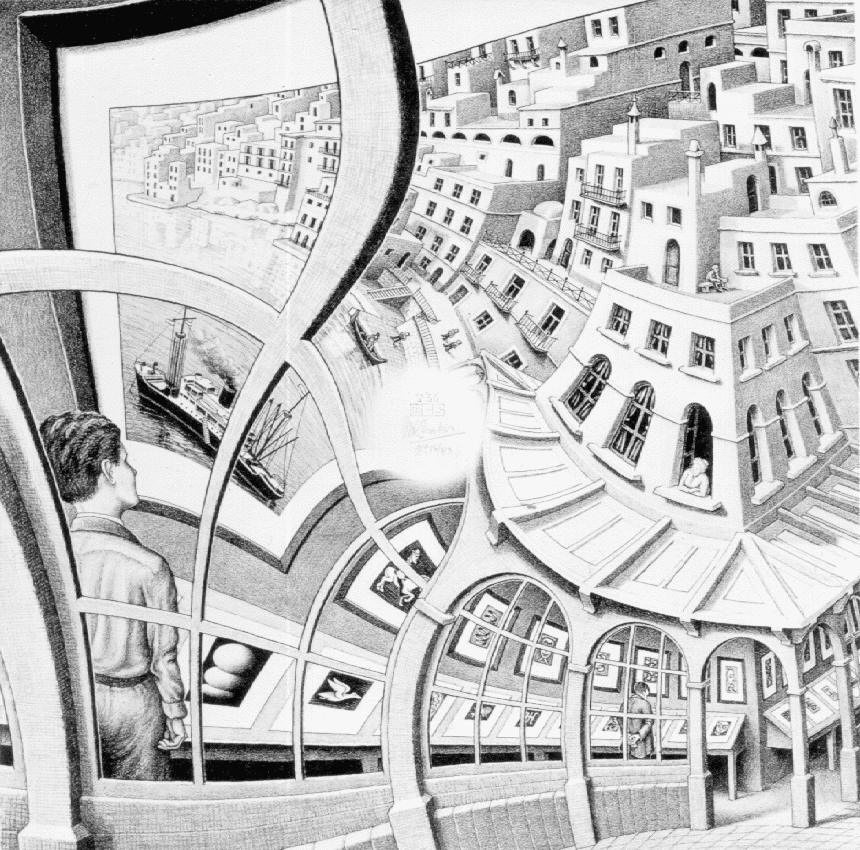
\includegraphics[width=0.3\columnwidth]{galleria_stampe.jpg} 
	\captionsource{A floating figure}{A floating figure: the lithograph \emph{Galleria di stampe}, of M.~Escher}{\url{http://www.mcescher.com/}}
	\label{fig:galleria} 
\end{figure}

\begin{figure}[H]
	\centering
	\begin{subfigure}[b]{0.45\textwidth}
		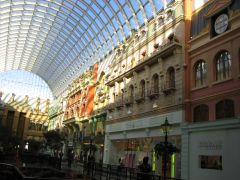
\includegraphics[width=\textwidth]{lorem.jpg}
		\caption{A gull}
		\label{fig:lorem}
	\end{subfigure}
	~ %add desired spacing between images, e. g. ~, \quad, \qquad, \hfill etc. 
	%(or a blank line to force the subfigure onto a new line)
	\begin{subfigure}[b]{0.45\textwidth}
		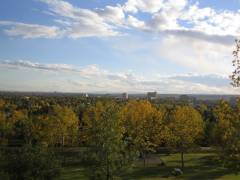
\includegraphics[width=\textwidth]{ipsum.jpg}
		\caption{A tiger}
		\label{fig:ipsum}
	\end{subfigure}
	~ %add desired spacing between images, e. g. ~, \quad, \qquad, \hfill etc. 
	%(or a blank line to force the subfigure onto a new line)
	\begin{subfigure}[b]{0.45\textwidth}
		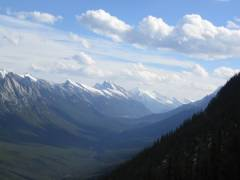
\includegraphics[width=\textwidth]{dolor.jpg}
		\caption{A mouse}
		\label{fig:dolor}
	\end{subfigure}
	~ %add desired spacing between images, e. g. ~, \quad, \qquad, \hfill etc. 
	%(or a blank line to force the subfigure onto a new line)
	\begin{subfigure}[b]{0.45\textwidth}
		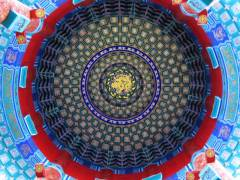
\includegraphics[width=\textwidth]{sit.jpg}
		\caption{A mouse}
		\label{fig:sit}
	\end{subfigure}
	\caption{Example subcaption}\label{fig:animals}
\end{figure}


% -----------------------------------------------------------------------------
\section{Code}

\autoref{lst:listing_example} shows an example of Java code rendered with minted.

\begin{listing}[H]
	\javafile{structure/listings/HelloWorld.java}
	\caption{Example of listing using the minted package}
	\label{lst:listing_example}
\end{listing}

% -----------------------------------------------------------------------------
\section{Other features}

Term (glossaries): \gls{nosql}

Acronym (glossaries): \gls{sql}

Citation (biblatex): \cite{paper_millwheel}

% -----------------------------------------------------------------------------
\section{Conclusion}

\blindtext

\chapter{Design}
\label{chap:design}

\lipsum[1]

\minitoc

\newpage

% -----------------------------------------------------------------------------
\section{Short lists}

\blindtext

\blindlist{enumerate}

\blindtext

\blindtext

\blindlist{itemize}

\blindtext

\blinddescription

% -----------------------------------------------------------------------------
\section{Long lists}

\blindtext

\Blindlist{enumerate}

\blindtext

\Blindlist{itemize}

\blindtext

\Blinddescription

% -----------------------------------------------------------------------------
\section{Multi-level lists}

\blindtext

\blindlistlist[3]{itemize}

\blindtext

\blindlistlist[3]{enumerate}

% -----------------------------------------------------------------------------
\section{Conclusion}

\lipsum[6-7]

\chapter{Implementation}
\label{chap:implementation}

\lipsum[1]

\minitoc

\newpage

% -----------------------------------------------------------------------------
\section{Section 1}

\lipsum[1-2]

% -----------------------------------------------------------------------------
\section{Section 2}


% -----------------------------------------------------------------------------
\section{Conclusion}

\chapter{Validation}
\label{chap:validation}

\lipsum[1]

\minitoc

\newpage

% -----------------------------------------------------------------------------
\section{Section 1}

\lipsum[2-4]

% -----------------------------------------------------------------------------
\section{Section 2}

\lipsum[4-7]

% -----------------------------------------------------------------------------
\section{Conclusion}

\lipsum[8-9]
\chapter{Conclusions}
\label{chap:conclusions}

% -----------------------------------------------------------------------------
\section{Project summary}

% -----------------------------------------------------------------------------
\section{Comparison with the initial objectives}

% -----------------------------------------------------------------------------
\section{Encountered difficulties}

% -----------------------------------------------------------------------------
\section{Future perspectives}


% Appendices
\chapter*{History}
\addcontentsline{toc}{chapter}{Version history}

\begin{table}[H]
    \hspace*{-0.7cm}
    \centering
    \rowcolors{1}{platinum}{white}
    \begin{tabular}{|L{2cm}|L{4cm}|L{8cm}|}
	\hline
	\rowcolor{languidlavender!80!gray} \textbf{\large{Version}} & \textbf{\large{Date}} & \textbf{\large{Modification}} \\
	\hline
        0.0 & - & - \\
        \hline
        \version & - & - \\
        \hline
    \end{tabular}
    \caption{Version history}
\end{table}
\appendix
\chapter{Appendices}

\lipsum[5-8]


% -----------------------------------------------------------------------------
% Back matter
% -----------------------------------------------------------------------------
\backmatter

% Bibliography
\cleardoublepage
\printbibliography[title={References}, heading=bibintoc]

% Glossary
\clearpage
\printglossaries

% TODO: Add index

% Add your CV here if you want

\end{document}
